%%%%%%%%%%%%%%%%%%%%%%%%%%%%%%%%%%%%%%%%%%%%
%%%%%%%%%%%%%%%%%%%%%%%%%%%%%%%%%%%%%%%%%%%%
\section{Background}

\begin{frame}
      \frametitle{Table of Contents}
      \tableofcontents[currentsection]
  \end{frame}


%%%%%%%%%%%%%%%%%%%%%%%%%%%%%%%%%%%%%%%%%%%%%%%%%%%%%%%%
{
{
\paper{
Wright-Gilbertson M. 2014 in PhD thesis
}

\begin{frame}{Optimal scanning plan for fetal US biometry}
      \begin{figure}
        \centering
        \includegraphics[width=1.0\textwidth]{optimal-scanning-plane/outputs/drawing-v00}
        % \caption{The sonographer-probe-patient control system}
      \end{figure}
\end{frame}
}




%%%%%%%%%%%%%%%%%%%%%%%%%%%%%%%%%%%%%%%%%%%%
%%%%%%%%%%%%%%%%%%%%%%%%%%%%%%%%%%%%%%%%%%%%
\section{Robotic Ultrasound-Guidance Procedures}
\begin{frame}
      \frametitle{Table of Contents}
      \tableofcontents[currentsection]
  \end{frame}


%%%%%%%%%%%%%%%%%%%%%%%%%%%%%%%%%%%%%%%%%%%%%%%%%%%%%%%%
{
\paper{
Ipsen et al. in Physics in Medicine and Biology 2021;
von Haxthausen et al. in Current Robotics Reports 2021;
Gerlach et al. in International Journal of Computer Assisted Radiology and Surgery 2022;
}

\begin{frame}{Robotic Ultrasound-Guidance Procedures}
      \begin{figure}
        \centering
        \includegraphics[width=1.0\textwidth]{robotic-us-guidance-procedures/outputs/drawing-v00}
        % \caption{The sonographer-probe-patient control system}
      \end{figure}
\end{frame}
}


%%%%%%%%%%%%%%%%%%%%%%%%%%%%%%%%%%%%%%%%%%%%
%%%%%%%%%%%%%%%%%%%%%%%%%%%%%%%%%%%%%%%%%%%%
\section{Framework for sonographer skill transfer learning}
\begin{frame}
      \frametitle{Table of Contents}
      \tableofcontents[currentsection]
\end{frame}

%%%%%%%%%%%%%%%%%%%%%%%%%%%%%%%%%%%%%%%%%%%%%%%%%%%%%%%%
{
\paper{
Leung T. Y. and Xochicale M. in RAMI-ICRA2023 \faGithub \hspace{0em} \url{https://github.com/mxochicale/rami-icra2023}
}

\begin{frame}{Framework for sonographer skill transfer learning}{}

      \begin{figure}
        \centering
        \includegraphics[width=1.0\textwidth]{framework/outputs/drawing-v00}
        % \caption{The sonographer-probe-patient control system}
      \end{figure}
\end{frame}
}



%%%%%%%%%%%%%%%%%%%%%%%%%%%%%%%%%%%%%%%%%%%%
%%%%%%%%%%%%%%%%%%%%%%%%%%%%%%%%%%%%%%%%%%%%
\section{Experiments: Design and Results}
\begin{frame}
      \frametitle{Table of Contents}
      \tableofcontents[currentsection]
  \end{frame}

%%%%%%%%%%%%%%%%%%%%%%%%%%%%%%%%%%%%%%%%%%%%%%%%%%%%%%%%
{
\paper{
Leung T. Y. and Xochicale M. in RAMI-ICRA2023 \faGithub \hspace{0em} \url{https://github.com/mxochicale/rami-icra2023}
}

\begin{frame}{Results of participant 01 (non-clinician)}{}

      \begin{figure}
        \centering
        \includegraphics[width=1.0\textwidth]{results-p01/outputs/drawing-v00}
        % \caption{The sonographer-probe-patient control system}
      \end{figure}
\end{frame}
}


%%%%%%%%%%%%%%%%%%%%%%%%%%%%%%%%%%%%%%%%%%%%%%%%%%%%%%%%
{
\paper{
Leung T. Y. and Xochicale M. in RAMI-ICRA2023 \faGithub \hspace{0em} \url{https://github.com/mxochicale/rami-icra2023}
}

\begin{frame}{Results of participant 02 (clinician)}{}
      \begin{figure}
        \centering
        \includegraphics[width=1.0\textwidth]{results-p02/outputs/drawing-v00}
        % \caption{The sonographer-probe-patient control system}
      \end{figure}
\end{frame}
}


%%%%%%%%%%%%%%%%%%%%%%%%%%%%%%%%%%%%%%%%%%%%
%%%%%%%%%%%%%%%%%%%%%%%%%%%%%%%%%%%%%%%%%%%%
\section{Conclusions and Future Work}
\begin{frame}
      \frametitle{Table of Contents}
      \tableofcontents[currentsection]
  \end{frame}


%%%%%%%%%%%%%%%%%%%%%%%%%%%%%%%%%%%%%%%%%%%%%%%%%%%%%%%%
{

\paper{
Leung T. Y. and Xochicale M. in RAMI-ICRA2023 \faGithub \hspace{0em} \url{https://github.com/mxochicale/rami-icra2023}
}

\begin{frame}{Conclusions and Future Work}

\begin{itemize}
\item We have presented a simple framework of skill transfer learning for robotic ultrasound-guidance procedures.
\item We presented sensor fusion methods and sampling rate techniques for optimal scanning plane of the four-chamber
view from two participants (one experienced clinician and one with little to none experience).
\item The experienced clinician showed a smother and quicker procedure compare to the lengthy and non-constant movement of the participant with little experience.
\item For future work, we pointed out the need of pruned and quantised neural network models
for real-time applications in robotic ultrasound-guidance procedure.
\end{itemize}

\end{frame}
}

